\documentclass{article}
\usepackage[pdftex]{graphicx}
\usepackage{graphics}
\usepackage{color}
\usepackage{url}

\begin{document}

\author{Karsten Loesing\\{\tt karsten@torproject.org}}
\title{Case study:\\Learning whether a Tor bridge is blocked\\by looking
at its aggregate usage statistics\\-- Part one --}
\maketitle

\section{Introduction}

Tor bridges\footnote{\url{https://www.torproject.org/docs/bridges}} are
relays that are not listed in the main directory.
Clients which cannot access the Tor network directly can try to learn a
few bridge addresses and use these bridges to connect to the Tor network.
Bridges have been introduced to impede censoring the Tor network, but in
the past we experienced successful blocking of bridges in a few countries.

In this report we investigate whether we can learn that a bridge is
blocked in a given country only by looking at its reported aggregate
statistics on usage by country.
By knowing that a bridge is blocked, we can, for example, avoid giving
out its address to users from that country.

Learning whether a bridge is blocked is somewhat related to our recent
efforts to detect censorship of direct access to the Tor
network.\footnote{\url{https://metrics.torproject.org/papers/detector-2011-09-09.pdf}}
The main difference is that we want to know which bridges are blocked and
which are not, whereas we don't care which relays are accessible in the
case of blocked direct access.
It's easy to block all relays, but it should be difficult to block all
bridges.

This report can only be seen as a first step towards researching bridge
blocking.
Even if a bridge reports that it had zero users from a country, we're
lacking the confirmation that the bridge was really blocked.
There can be other reasons for low user numbers which may be completely
unrelated.
The results of this analysis should be considered when actively scanning
bridge reachability from inside a country, both to decide how frequently a
bridge should be scanned and to evaluate how reliable an analysis of
passive usage statistics can be.

\section{Bridge usage statistics}

Bridges report aggregate usage statistics on the number of connecting
clients.
Bridges gather these statistics by memorizing unique IP addresses of
connecting clients over 24 hour periods and resolving IP addresses to
country codes using an internal GeoIP database.
Archives of these statistics are available for analysis from the metrics
website.\footnote{\url{https://metrics.torproject.org/data.html#bridgedesc}}
Figure~\ref{fig:bridgeextrainfo} shows an example of bridge usage
statistics.
This bridge observed 41 to 48 connecting clients from Saudi Arabia
(all numbers are rounded up to the next multiple of 8), 33 to 40
connecting clients from the U.S.A., 25 to 32 from Germany, 25 to 32 from
Iran, and so on.
These connecting clients were observed in the 24~hours (86,400 seconds)
before December 27, 2010, 14:56:29 UTC.

\begin{figure}[h]
\begin{quote}
\begin{verbatim}
extra-info Unnamed A5FA7F38B02A415E72FE614C64A1E5A92BA99BBD
published 2010-12-27 18:55:01
[...]
bridge-stats-end 2010-12-27 14:56:29 (86400 s)
bridge-ips sa=48,us=40,de=32,ir=32,[...]
\end{verbatim}
\end{quote}
\caption{Example of aggregate bridge usage statistics}
\label{fig:bridgeextrainfo}
\end{figure}

An obvious limitation of these bridge usage statistics is that we can only
learn about connecting clients from bridges with at least 24 hours uptime.
It's still unclear how many bridge users are not included in the
statistics because of this, which is left for a different analysis.

We further decided to exclude bridges running Tor versions 0.2.2.3-alpha
or earlier.
These bridges report similar statistics as the later Tor versions that
we're considering here, but do not enforce a measurement interval of
exactly 24 hours which would have slightly complicated the analysis.
We don't expect the bridge version to have an influence on bridge usage
or on the likelihood of the bridge to be blocked in a given country.

\section{Case study: China in the first half of 2010}

The major limitation of this analysis is that we don't have the data
confirming that a bridge was actually blocked.
We may decide on a case-by-case basis whether a blocking is a plausible
explanation for the change in observed users from a given country.
Anything more objective requires additional data, e.g., data obtained from
active reachability scans.

We decided to investigate bridge usage from China in the first half of
2010 as a case study.
Figure~\ref{fig:bridge-users} shows estimated daily bridge users from China
since July 2009.
The huge slope in September and October 2009 is very likely a result from
China blocking direct access to the Tor network.
It seems plausible that the drops in March and May 2010 result from
attempts to block access to bridges, too.
We're going to focus only on the interval from January to June 2010 which
promises the most interesting results.
We should be able to detect these blockings in the reported statistics of
single bridges.
Obviously, it may be hard or impossible to transfer the findings from this
case study to other countries or situations.

\begin{figure}
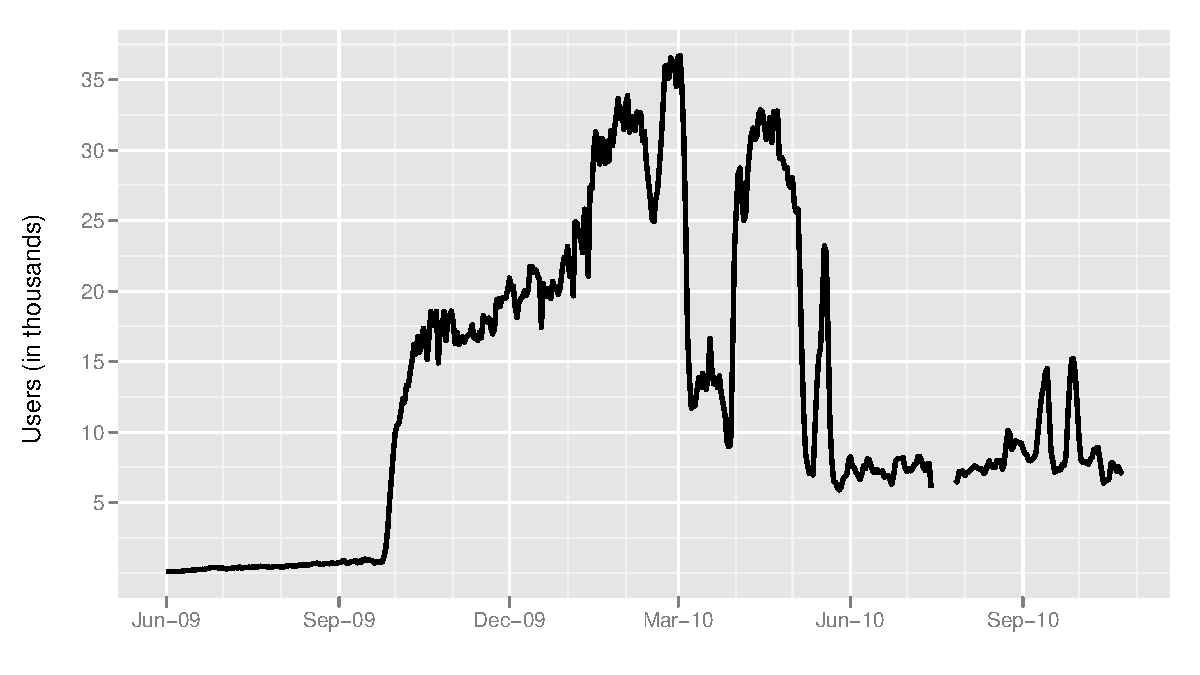
\includegraphics[width=\textwidth]{bridge-users.png}
\caption{Estimated daily bridge users from China}
\label{fig:bridge-users}
\end{figure}

\paragraph{Definition of bridge blocking}

We have a few options to define when we consider a bridge to be blocked
from a given country on a given day.

\begin{itemize}
\item \textbf{Absolute threshold:}
The absolute number of connecting clients from a country falls below a
fixed threshold.
\item \textbf{Relative threshold compared to other countries:}
The fraction of connecting clients from a country drops below a fixed
percent value.
\item \textbf{Estimated interval based on history:}
The absolute or relative number of connecting clients falls outside an
estimated interval based on the recent history.
\end{itemize}

For this case study we decided to stick with the simplest solution being
an absolute threshold.
We define a somewhat arbitrary threshold of 32 users to decide whether a
bridge is potentially blocked.
A blocked bridge does not necessarily report zero users per day.
A likely explanation for reporting users from a country that blocks a
bridge is that our GeoIP is not 100~\% accurate and reports a few users
which in fact come from other countries.

The reason against using a relative threshold was that it depends on
development in other countries.
As we can see in the example of China, bridge usage can depend on the
abilty to directly access the Tor network.
A sudden increase in country $A$ could significantly lower the relative
usage in country $B$.
We should probably consider both absolute and relative thresholds in
future investigations.
Maybe we also need to take direct usage numbers into account.

We also didn't build our analysis upon an estimated interval based on the
recent history, because it's unclear how fast a bridge will be blocked
after being set up.
If it only takes the censor a few hours, the bridge may never see much use
from a country at all.
An estimate based on the bridge's history may not detect the censorship at
all, because it may look like a bridge with only few users from that
country.

We plan to reconsider other options for deciding that a bridge is blocked
once we have data confirming this.

\paragraph{Visualization of bridge blockings}

Figure~\ref{fig:bridge-blockings} shows a subset of the raw bridge usage
statistics for clients connecting from China in the first half of 2010.
Possible blocking events are those when the bridge reports 32 or fewer
connecting clients per day.
These events are marked with red dots.

We decided to only include bridges in the figure that report at least
100~Chinese clients on at least one day in the whole interval.
Bridges with fewer users than that have a usage pattern that makes it much
more difficult to detect blockings at all.
The figure also shows only bridges reporting statistics on at least 30
days in the measurement interval.

\begin{figure}[t]
\includegraphics[width=\textwidth]{bridge-blockings.png}
\caption{Subset of bridge usage statistics for Chinese clients in the
first half of 2010}
\label{fig:bridge-blockings}
\end{figure}

The single bridge usage plots indicate how difficult it is to detect
blockings only from usage statistics.
About 10 of the displayed 27 plots have a pattern similar to the expected
pattern from Figure~\ref{fig:bridge-users}.
The best examples are probably bridges \verb+C037+ and \verb+D795+.
Interestingly, bridge \verb+A5FA+ was unaffected by the blocking in March
2010, but affected by the blocking in May 2010.

\paragraph{Aggregating blocking events}

As the last step of this case study we want to compare observed bridge
users to the number of blocked bridges as detected by our simple threshold
approach.
We would expect most of our bridges to exhibit blockings in March 2010 and
from May 2010 on.
Figure~\ref{fig:bridge-users-blockings} plots users and blocked bridges
over time.
The two plots indicate that our detection algorithm is at least not
totally off.

\begin{figure}[t]
\includegraphics[width=\textwidth]{bridge-users-blockings.png}
\caption{Estimated users and assumed bridge blockings in China in the
first half of 2010}
\label{fig:bridge-users-blockings}
\end{figure}

\section{Conclusion}

Passively collected bridge usage statistics seem to be a useful tool to
detect whether a bridge is blocked from a country.
However, the main conclusion from this analysis is that we're lacking the
data to conduct it usefully.
One way to obtain the data we need are active scans.
When conducting such scans, passively collected statistics may help reduce
the total number and frequency of scans.
For example, when selecting a bridge to scan, the reciprocal of the last
reported number of connecting clients could be used as a probability
weight.
Once we have better data confirming bridge blocking we shall revisit the
criteria for deriving the blocking from usage statistics.

\end{document}

